\documentclass[xetex,mathserif,serif]{beamer}

\usetheme{Darmstadt}
\usecolortheme{beetle}

\usepackage{graphicx}
\makeatletter
\providecommand{\bigsqcap}{%
  \mathop{%
    \mathpalette\@updown\bigsqcup
  }%
}
\newcommand*{\@updown}[2]{%
  \rotatebox[origin=c]{180}{$\m@th#1#2$}%
}
\makeatother


\title % (optional, only for long titles)
{Apstraktna interpretacija u modernim kompajlerima}
\subtitle{Seminarski rad u okviru kursa Metodologija stručnog i naučnog rada}
\author[Demonja, Maksimović, Crnobrnja] % (optional, for multiple authors)
{O.~Demonja, S.~Maksimović i M.~Crnobrnja}
\institute% (optional)
{
  Matematički fakultet\\
  Univerzitet u beogradu
}
\date % (optional)



\begin{document}
  \frame{\titlepage}
  \begin{frame}
    \frametitle{Formalizacija}
	    \framesubtitle{Skupovi konkretnih i apstraktnih stanja}
		\begin{center}
			\begin{itemize}
				\item $v \in V$ skup konkretnih stanja
				\item $v_{1} \rightsquigarrow v_{2}$ relacija prelaska
				\item $... \rightsquigarrow v_{n} \rightsquigarrow v_{n}$ zaustavljanja programa
				\item $l \in L$ prostor svojstava
				\item $l_{1} \rightarrow l_{2}$ \emph{funkcija} prelaska
				\item $\sqsubseteq \; \; \subset \; L \times L$ relacija poretka nad $L$
				\begin{itemize}
					\item $a \sqsubseteq a$ refleksivnost
					\item $a \sqsubseteq b \wedge b \sqsubseteq a \implies a = b$ antisimetričnost
					\item $a \sqsubseteq b \wedge b \sqsubseteq c \implies a \sqsubseteq c$ tranzitivnost
				\end{itemize}
				\item potpuna mreža
				\begin{itemize}
					\item $\forall l_0 \in L^{\prime} \; \; l_0 \sqsubseteq \bigsqcup_{l \in L^{\prime}} l$
					\item $\forall l_0 (\forall l \in L^{\prime} \; l \sqsubseteq	l_0) \implies \bigsqcup_{l \in L^{\prime}} l \sqsubseteq l_0 $
					\item analogno za $\bigsqcap_{l \in L^{\prime}} l$ ...
				\end{itemize}
			\end{itemize}
		\end{center}
  \end{frame}
  \begin{frame}
    \frametitle{Formalizacija}
	    \framesubtitle{Skupovi konkretnih i apstraktnih stanja}
		\begin{center}
		    \begin{figure}
				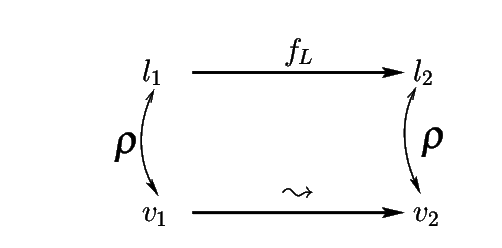
\includegraphics[scale=0.5]{Rho.png}
			\end{figure}
		\end{center}
  \end{frame}
  \begin{frame}
    \frametitle{Formalizacija}
    \begin{figure}
		\begin{center}
		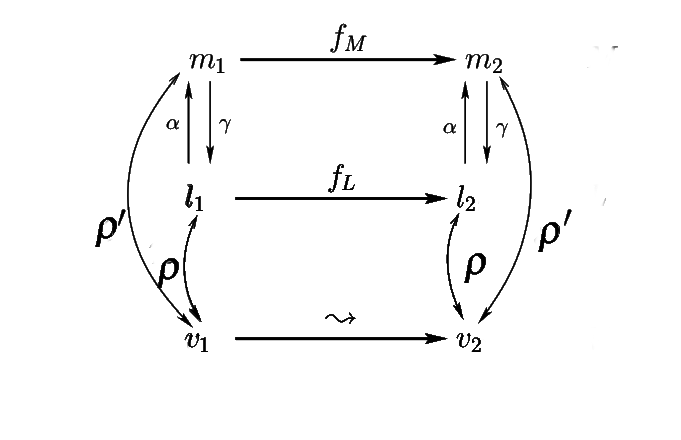
\includegraphics[scale=0.5]{Rho_prime.png}
		\end{center}
	\end{figure}
  \end{frame}
  \begin{frame}
    \frametitle{Formalizacija}
    \framesubtitle{Fiksne tačke}
	\begin{center}
		\begin{itemize}
			\item $x = f_{L}(x)$
			\item Čine potpunu mrežu.
		\end{itemize}
		\end{center}
  \end{frame}
  %
  \begin{frame}
    \frametitle{Primeri}
    \framesubtitle{Uvod}
    \begin{center}
		\begin{itemize}
			\item Uglavnom intraproceduralna apstraktna interpretacija - vr\v si se za svaku funkciju posebno
			\begin{itemize}
				\item Tra\v zenje konstantnih varijabli
				\item Dereferenciranje null pokaziva\v ca
				\item Inicijalizacija promenljivih koje se kasnije koriste
				\item \emph{lock/unlock, fopen/fclose}
			\end{itemize}
			\item Primer na problemu \emph{propagacije konstanti}
			\begin{itemize}
				\item Prolaz kroz funkciju koriste\v ci apstraktne vrednosti kao ulaz 
				\item Apstraktna vrenost predstavlja skup konkretnih vrednosti
				\item Kada imamo grananje, krenimo put obe grane
				\item Gde imamo spajanje, spajamo izlaz iz obe grane
			\end{itemize}
		\end{itemize}
	\end{center}
  \end{frame}
  \begin{frame}
    \frametitle{Primeri}
    \framesubtitle{Graf kontrole toka, CFG}
    \begin{figure}
		\begin{center}
		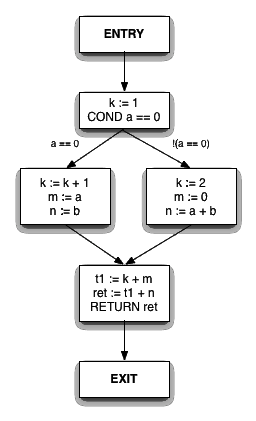
\includegraphics[scale=0.5]{Treehydra-cfg.png}
		\end{center}
	\end{figure}
  \end{frame}
  \begin{frame}
    \frametitle{Primeri}
    \framesubtitle{Karakteristike apstraktne interpretacije}
	\begin{center}
		\begin{itemize}
			\item Ta\v cnost i pouzdanost
				\begin{itemize}
					\item Stati\v cka analiza nije savr\v sena, moramo praviti kompromis
					\item Vr\v senje stro\v zijih provera, prijavljivanje la\v znih pozitiva
					\item Bla\v ze provere, \v sansa da nam promaknu neke gre\v ske
				\end{itemize}
			\item Cena
				\begin{itemize}
					\item Algoritmi u najgorem slu\v caju eksponencijalne slo\v zenosti
					\item Dosta se sporije vi\v si od procesa prevo\dj{}enja
				\end{itemize}
		\end{itemize}
	\end{center}
  \end{frame}
  
% etc
\end{document}
